\documentclass[9pt]{extarticle}

\usepackage[utf8]{inputenc}
\usepackage[english]{babel}
\usepackage{hyperref}
\usepackage{extsizes}
\usepackage{caption}
\usepackage{subcaption}
\usepackage[table,dvipsnames]{xcolor}
\definecolor{lgray}{gray}{0.95}

\usepackage[square,numbers]{natbib}
\bibliographystyle{plainnat}
\setcitestyle{authoryear,open={(},close={)}}

\usepackage{amsfonts, amsmath, amssymb, amsthm}

\newtheorem{theorem}{Theorem}[section]

\usepackage{graphicx}
\usepackage{float}

\usepackage[margin=1in]{geometry}

\usepackage[utf8]{inputenc}
\usepackage{fancyhdr}
 
\pagestyle{fancy}
\fancyhf{}


\renewcommand{\headrulewidth}{1.5pt}% 2pt header rule
\renewcommand{\headrule}{\hbox to\headwidth{%
		\color{MidnightBlue}\leaders\hrule height \headrulewidth\hfill}}
\renewcommand{\footrulewidth}{0pt}% No footer rule
%\renewcommand{\footrule}{\hbox to\headwidth{%
%		\color{MidnightBlue}\leaders\hrule height \footrulewidth\hfill}}


\rhead{Benjamin Cox}
\chead{Statistical Consultancy -- Assessment 2}
\lhead{Due 22nd November}
\cfoot{Page \thepage}

\begin{document}

\section{Introduction}

We consider data on the survival of passengers of the RMS Titanic. The data contains many variables about the passengers of the Titanic, some of which we will use and some of which we will not. We are going to perform logistic regression in order to ascertain the effect that certain variables have on the survival of a passenger. We have 1309 individual passenger records to analyse. 

We are particularly interested in the affect of socio-economic status on survival probabilities, as well as whether the adage of `women and children first' holds.

\section{Statistical Analysis}

\subsection{Introduction to our data}

The survival variable is binary (they either survived or died). This is the reason for using simple logistic regression. The passenger class is a factor variable with three levels corresponding to 1st, 2nd, and 3rd class. The sex is a factor variable with two levels corresponding to male and female. The age is a continuous variable (with rounding applied). We have data on the sum number of siblings and spouses aboard of a passenger, as well as of the number of parents and children. These are highly correlated, so we will only use one. In our case we will use the siblings and spouses. We have the ticket number, which is useless for our analysis. We have the fare paid by the passenger. This is continuous and has properties that warrant a discussion later. We have the cabin number, which we will use to ascertain whether a passenger had a cabin (this is highly correlated with passenger class). We have the port of embarkation, which is one of Cherbourg, Queenstown, and Southampton. We have the lifeboat number, which is useless, as well as the body number. These are both useless as they are a posteriori of the survival. We also have the home/destination of the passenger. This is also useless.

This time around our data has no missingness that is not appropriate. Moreover none of the variables that we are analysing have missingness (the NA in cabin number means that the passenger did not have a cabin). 

\subsection{Initial Analysis}

We first need to conduct an analysis of the independence of the variables we think we may include in our model. Performing a chi squared test we find that most variables of interest for the model are highly interdependent. However the type of model that we are fitting is somewhat resilient to this. What is important is that the variables are not co-linear. Most of our variables cannot be co-linear as they are factor variables. The only ones of concern are the sum number of siblings and spouses and the sum number of parents and children. We calculate the variance inflation factors for these variables. They come out as 1.24 and 1.23 respectively. The standard threshold for multicollinearity is 3, so we are very safe.

Looking at the fare paid by the passenger it is clear that in our data the fare paid is that of the ticket purchase, not per person. This means that those travelling in large groups will seem to pay a very large fare, whilst in reality no paying quite so high a price. Couple this with the fact that the fare is inextricably linked with both the passenger class and whether the passenger received a cabin and we are safe to remove this factor from our model. 

We will also note that there are some mistakes in the data; some ages are recorded incorrectly. As there are thousands of records we hope that the correct values will swamp the effect of the incorrect values. No attempt will be made to fix the data, as there is no reasonable way to do so in the time-frame given for this analysis.

The data that we have been provided has been subject to imputation. This was particularly heavy in the age variable, with 263 values being imputed. As we have only the one dataset we cannot bring to bear many of the tools that are available to deal with the uncertainty brought about by missing data imputation. We must simply keep in mind that the statistics for age will be artificially more certain.

Both of the above are immaterial for our analysis however; we have been given a dataset and instructed to analyse it. The data could be completely fictional and the method of analysis would not change. We are merely pointing this out to provide some additional context for our reader.

\subsection{Model Design}

We are going to use a logistic regression with the response variable being the logit probability of survival. This means that the response variable is of the form $y = \ln(P/1-P),$ where $P$ is the probability of survival. We do this as we are modelling a categorical variable, so we want a response that is close to categorical. We can simply round the response to get an indicator as to whether the passenger would likely survive or perish.

We create the model with the predictors being age, sex, class, port of embarkation, whether or not the passenger had a cabin, and the sum number of siblings and spouses the passenger had aboard (hereon referred to as sibsp).

The reason for excluding the sum number of parents and children of the passenger is that it is extremely closely interlinked with the age and sibsp. It does not add much to the model when included as the corresponding coefficient is not statistically significantly different from 0.

We could include a parsed title of the passenger as a factor variable, however the overwhelming majority of the passengers go by the one of standard three (Mr., Mrs., Miss.). This means that this would be highly susceptible to outliers, as well as being completely dependent on sex.

We do not include fare as it is completely dependent on class and the number of people travelling in a certain party. An example would be the wealthy Sir Duff Gordon's fare being recorded as 56.93 pounds, and the 3rd class passenger Mr Frederick Sage having his fare recorded as 69.55 pounds. This is due to his travelling in a party of 11. This means that this should be accounted for by passenger class and sibsp.

We make the cabin into a binary variable. The idea for this is that people with a cabin are likely to have easier access to the decks to evacuate. We note that not all 1st class passengers had cabins, and not all cabins were 1st class. This makes it quite the interesting predictor.

We are instructed to include interaction terms for age-sex and age-pclass, so determine whether age has a different effect depending on these variables.

One thing that is of note is the relative uselessness of standard diagnostic plots when applied to a logistic regression model. We see in Figure \ref{fig:modeldiag} that the plots look as though something is amiss. This is not the case. The residual-fitted plot looks as though we have missed some sort of curvilinear trend. This is not the case; logistic regression is curvilinear by nature, so the trend displayed is perfectly fine. The residual-leverage plot looks mostly fine, however outliers do not manifest in the same way as linear regression, so the plot may not be of much use in identifying them. The Q-Q plot looks quite bad, but logistic regression models do not require normality of residuals to be valid. The most useful one is Cook's distance, which helps use estimate the relative importance of a point in the regression. What we have looks perfectly fine, so we do not need to worry.

\section{Discussion of Results}

Graphs showing the predicted survival by age with variable class and sex are given in Figure \ref{fig:psurvage}. We see that women had a far greater chance of survival than men of the same class. In fact 3rd class women had a better survival chance than 1st class men. This, coupled with the decreasing survival probabilities with age, points to `women and children first' very much being obeyed. 

We check our predicted against our actual and get that the model that we have fitted is 80.60\% accurate in this case (meaning that it is correct 80.60\% of the time). 

More explicitly we have that the coefficients for the model are found in Table \ref{tab:regco}. Note that these effect the logit of the probability (as given above), so we need to invert this in order to get the predicted probability of survival. The predicted probability of survival is given by $P_{surv} = \exp(y)/(1+\exp(y)),$ where $y$ is our response variable.
\subsection{Effect of Age}

We see that Table \ref{tab:regco} gives the coefficient for age as $0.03$ for females and $-0.08$ for males. The female effect is eclipsed by other effects and it's own error, and when only age and class is accounted for is not present. This is reflected in the plots in Figure \ref{fig:psurvage}. We see that the predicted survival probabilities start out relatively high but decrease quite quickly.

We also see that age had a different effect based on passenger class. It is, predictably, a worse effect for 2nd and 3rd class than for 1st. Of note is that the effect for 2nd class is more severe and more significant than that for 3rd class.

\subsection{Effect of Gender}

We see that the logit probability for a male is $0.48$ lesser than that of an equivalent female. This is also reflected in the plots in Figure \ref{fig:psurvage}. The predicted survival probabilities for males are significantly lower overall, and especially so for adults. We note that we do not have data for the crew. Having this data would likely further decrease the odds of male survival, as a majority of the crew was male and died.

\subsection{Effect of Class}

In Table \ref{tab:regco} we see that the predicted logit probability of survival for a 2nd class passenger is $0.81$ more than that of a 1st class passenger. For a third class passenger the difference is $-0.32$ less. This shows that there is a clear link between passenger class and survival probabilities. This is clearly reflected in Figure \ref{fig:psurvage}. We see that the 3rd class survival probabilities are significantly inferior to those of their 1st and 2nd class counterparts. This points to a clear trend with regards to socio-economic status and survival chances. This also reflects the effect that the relatively small number of 2nd class passengers has on our model. When this variable is accounted for individually the effects are as expected; 1st class survives more than 2nd, 2nd more than 3rd. The interaction with age has a significant effect on the model.

\subsection{Effect of Cabin}

Table \ref{tab:regco} gives the increase in logit probability of survival of an individual having a cabin as $0.78$ compared to an equivalent individual who did not have a cabin. 
This is a significant increase in survival probabilities; the difference is more than that between 2nd and 1st class. This may have something to do with the location of the passenger and their ability to get above deck to abandon ship. 

\subsection{Effect of Port of Embarkation}

We see that in Table \ref{tab:regco} the logit survival of someone who boarded in Queenstown is $0.40$ lower than someone who boarded in Cherbourg. For a passenger who boarded in Southampton their logit survival is $0.58$ lower than if they boarded in Queenstown. This may be to do with the proportions of classes that boarded in each port; Cherbourg had more 1st class passengers board than all other combined. However Southampton had a representative mix, so this is up in the air. Perhaps it is to do with room allocation, we cannot truly know. The effect of Queenstown is not significant at the $5\%$ level, but is kept as the effect of Southampton is, so the comparison is warranted. All this means is that Cherbourg and Queenstown are likely to have comparable survivals.

\subsection{Effect of Sum Number of Siblings and Spouses}

We see that for each sibling or spouse a passenger has on board the logit survival decreases by $0.40$. We note that the vast majority of passengers had no siblings or spouses aboard, so this would not effect them. Of the rest, most had one, with numbers higher than this being rather rare. The highest recorded is 8, with none of these passengers surviving. This can be interpreted in a socio-economic sense, with the poor of the time having larger families. However, some passengers may have chosen to remain on board with their family, which is reflected in this statistic.

\section{Illustrative Examples}

In this section we will generate some example passengers and give the chances of survival for each of them. The data generated is given in Table \ref{tab:illdata}.

\subsection{1st Class Couple}

The first archetype is that of the first class couple. We make them relatively young, with a cabin and embarking at Cherbourg. They are represented in rows 1 and 2 of Table \ref{tab:illdata}. Given the data the female will most likely survive, however her partner has relatively even odds of survival. This is what we would typically think of when we think of maritime passengers in the early 1900s.

\subsection{3rd Class Family}

Another archetype is that of the third class family. They are represented by rows 3 to 7 of Table \ref{tab:illdata}. The father very likely perishes, with the mother most likely joining him. The two male children are also likely to die. The young female child is also more likely than not to die. This is what we expect, unfortunately.

\subsection{2nd Class Couple with Sister}

We generate a 2nd class couple with the wife bringing her sister. We make them a bit older this time. They are represented by rows 8, 9, and 10 in Table \ref{tab:illdata}. We see that the man is extremely likely to perish, with his partner being quite likely to survive. Her sister is even more likely to survive. This is illustrative of `women and children first`, as they are very similar in all aspects excepting sex. This also displays the effect of siblings and spouses quite nicely.

\section{Conclusion}

The Titanic was an unmitigated disaster. It shaped the protocols for passenger ship design for generations, as well as navigational procedures and search and rescue. It became an important cultural icon, uniting many in the idea of `what if?' The design of the ship was such that there were insufficient lifeboats, drills were not carried out to ensure passengers and crew knew how to react. The culture of the time shaped the survival of the passengers. 

We can only conclude that were there more lifeboats and proper training in the procedures for their use many more, if not all, would have survived. The incident is utterly damning of the attitudes of the time, as well as more concretely the shipbuilding methods. We see that the survivors were disproportionately upper class, with the vast majority of steerage and the crew perishing due to the ill designed ship, the poor command, and the shoddy preparation.

%\pagebreak
%\bibliography{references}

\appendix

\section{Plots and Figures}

\begin{figure}[H]
	\centering
	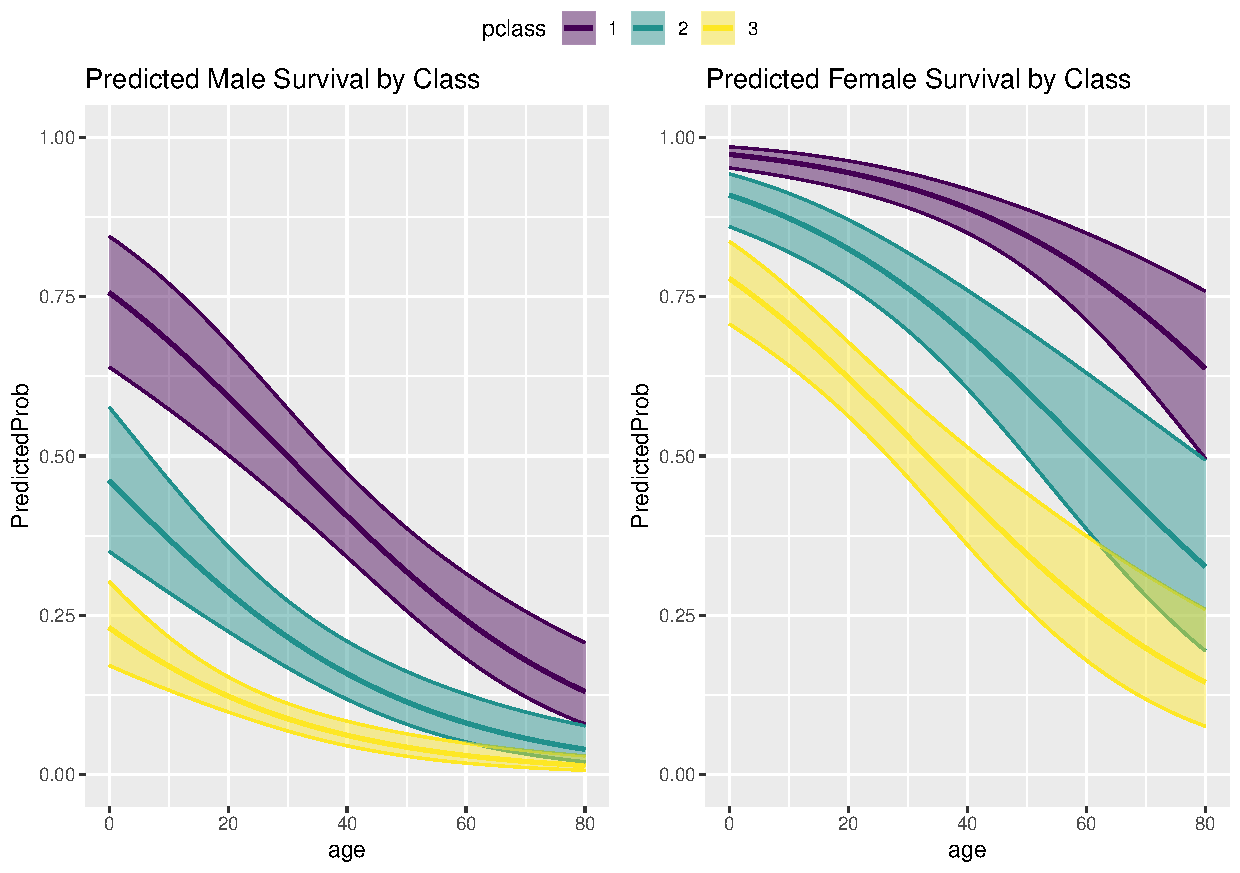
\includegraphics[width=0.6\textwidth]{psurvage}
	\caption{Predicted survival probabilities with 95\% prediction intervals}
	\label{fig:psurvage}
\end{figure}

\begin{figure}[H]
	\centering
	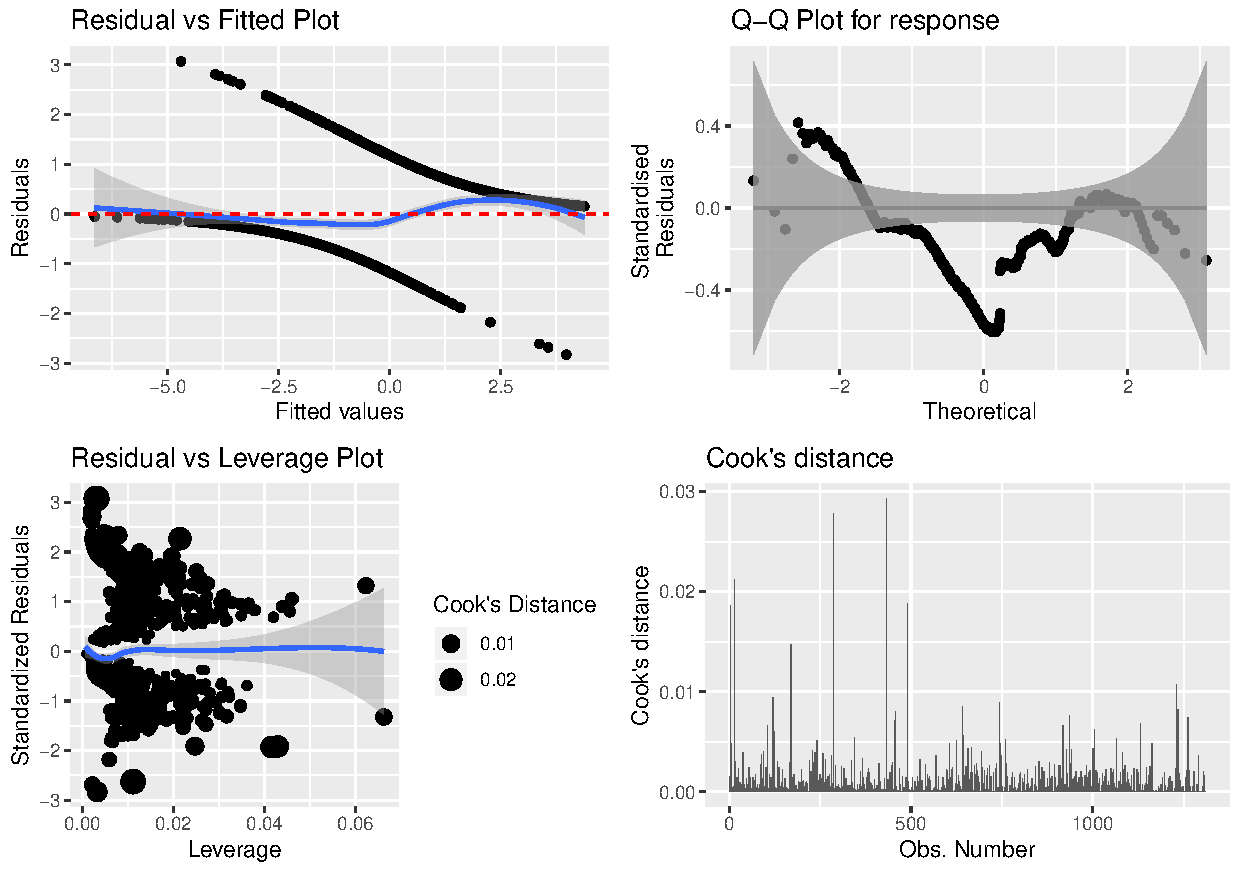
\includegraphics[width=0.6\textwidth]{modeldiag}
	\caption{Diagnostic plots for our model}
	\label{fig:modeldiag}
\end{figure}

\section{Tables}
\begin{table}[H]
	\centering
	\rowcolors{1}{white}{lgray}
	\begin{tabular}{rlrr}
		\hline
		& term & estimate & std.error \\ 
		\hline
		1 & (Intercept) & 1.65 & 0.62 \\ 
		2 & pclass2 & 0.81 & 0.66 \\ 
		3 & pclass3 & -0.32 & 0.60 \\ 
		4 & sexmale & -0.48 & 0.38 \\ 
		5 & age & 0.03 & 0.02 \\ 
		6 & sibsp & -0.40 & 0.09 \\ 
		7 & embarkedQ & -0.40 & 0.30 \\ 
		8 & embarkedS & -0.58 & 0.19 \\ 
		9 & cabinY & 0.87 & 0.28 \\ 
		10 & sexmale:age & -0.08 & 0.01 \\ 
		11 & pclass2:age & -0.05 & 0.02 \\ 
		12 & pclass3:age & -0.04 & 0.02 \\ 
		\hline
	\end{tabular}
\caption{Regression coefficients for the logistic fit}
\label{tab:regco}
\end{table}

\begin{table}[H]
	\centering
	\rowcolors{1}{white}{lgray}
	\begin{tabular}{rlllrrllr}
		\hline
		& pclass & survived & sex & age & sibsp & cabin & embarked & p\_surv \\ 
		\hline
		1 & 1 &  & male &  35 &   1 & Y & C & 0.48 \\ 
		2 & 1 &  & female &  28 &   1 & Y & C & 0.95 \\ 
		3 & 3 &  & male &  35 &   1 & N & S & 0.03 \\ 
		4 & 3 &  & female &  30 &   1 & N & S & 0.47 \\ 
		5 & 3 &  & male &  10 &   2 & N & S & 0.19 \\ 
		6 & 3 &  & male &  12 &   2 & N & S & 0.16 \\ 
		7 & 3 &  & female &   6 &   2 & N & S & 0.46 \\ 
		8 & 2 &  & male &  55 &   1 & Y & Q & 0.03 \\ 
		9 & 2 &  & female &  50 &   2 & Y & Q & 0.75 \\ 
		10 & 2 &  & female &  52 &   1 & Y & Q & 0.81 \\ 
		11 & 1 &  & male &  65 &   0 & Y & C & 0.25 \\ 
		12 & 3 &  & male &  22 &   1 & N & S & 0.10 \\ 
		13 & 3 &  & female &  20 &   1 & N & S & 0.51 \\ 
		14 & 1 &  & male &  32 &   1 & N & S & 0.20 \\ 
		15 & 1 &  & female &  26 &   1 & N & S & 0.81 \\ 
		16 & 1 &  & male &   6 &   1 & N & S & 0.48 \\ 
		17 & 1 &  & female &   4 &   1 & N & S & 0.69 \\ 
		\hline
	\end{tabular}
\caption{Illustrative examples of passenger archetypes}
\label{tab:illdata}
\end{table}
\end{document}